\documentclass{article}

\title{Fast and Flexible Variational Bayes for Sparse Binary Matrices}
%\author{Neil Houlsby}
\date{\today}

\usepackage{fullpage}
\usepackage{natbib}
\usepackage{amsmath}
\usepackage{amssymb}
\usepackage{graphicx}
\usepackage{color}

\newcommand{\obs}{O}
\newcommand{\X}{\mathbf{X}}
\newcommand{\A}{\mathbf{A}}
\newcommand{\s}{\mathbf{S}}
\newcommand{\Z}{\mathbf{Z}}
\newcommand{\N}{\mathcal{N}}
\newcommand{\T}{\mathcal{T}}
\newcommand{\atil}{\tilde{a}}
\newcommand{\abar}{\bar{a}}
\newcommand{\stil}{\tilde{s}}
\newcommand{\sbar}{\bar{s}}
\newcommand{\btil}{\tilde{b}}
\newcommand{\bbar}{\bar{b}}
\newcommand{\gtil}{\tilde{g}}
\newcommand{\gbar}{\bar{g}}
\newcommand{\ztil}{\tilde{z}}
\newcommand{\zbar}{\bar{z}}
\newcommand{\zetabar}{\bar{\zeta}}
\newcommand{\E}{\mathbb{E}}
\newcommand{\argmax}{ \operatorname*{arg \max}} 
\newcommand{\argmin}{ \operatorname*{arg \min}} 
\newcommand{\zua}{\left(\frac{u_s-\abar}{\sqrt{\atil}}\right)}
\newcommand{\zla}{\left(\frac{l_s-\abar}{\sqrt{\atil}}\right)}
\newcommand{\zus}{\left(\frac{u_s-\sbar}{\sqrt{\stil}}\right)}
\newcommand{\zls}{\left(\frac{l_s-\sbar}{\sqrt{\stil}}\right)}

\begin{document}

\maketitle

\begin{abstract}

\end{abstract}

\section{Introduction}
We seek to factorise the binary matrix $\X\in\mathbb{R}^{I\times J}$ whose elements are binary ($x_{ij}\in\{-1,+1\}$) as the product of two lower rank matrices $\A\in\mathbb{R}^{I\times K}$ and $\s\in\mathbb{R}^{K\times J}$, i.e. $\X = \A\s$.
We have observed only the elements $\obs$ from $\X$, of which we denote $\mathcal{O}^+$ and $\mathcal{O}^-$ the sets of $+1$s and $-1$s respectively.
These matrices are often sparse, i.e. $\mathcal{O}^+ \ll \mathcal{O}^-$.
Probilistic methods for this factorisation are popular because of their ability to handle noise in a formal manner, and deal with missing entries. 

However, performing Bayesian inference is intractable so Variational Bayes is used for approximate inference.
This may be solved analytically, as in \citep{nakajima2010}, or by gradient descent, as in \citep{raiko2007}.
The analytic solution has the advantage that it is faster, requiring only $O(\mathcal{O}^+)$ computations, however, it is more restrictive.
Additional complexity e.g. non-zero mean priors can be added in a straightforward manner to the gradient descent-based approach,
however, the complexity is $O(\mathcal{O})$ i.e. linear in the \emph{total} number of elements, rather than just the $+1$s.
Both these approaches use a Gaussian likelihood function, which is somewhat unsatisfactory for a binary matrix, where a classification likelihood would be expected to perform better.

Recent work has extended the analytic solution to arbitrary likelihood functions \citep{seeger2012}; however it performs some crude approximations and our experiments do not indicate
that it offers a large advantage over the Gaussian likelihood. 
In this work we extend the gradient descent approach to binary matrices seeking $O(\mathcal{O}^+)$ complexity.
We present both a solution for Gaussian and classification likelihoods.

In Section \ref{sec:gaussian} we present the current Gaussian gradient descent approach \citep{raiko2007}, in Section \ref{sec:sigmoid} we extend this to a Sigmoidal likelihood. 
We reduce the complexity to $O(\mathcal{O}^+)$ in Section \ref{sec:sparse} and demonstrate the performance of the algorithm on some large matrices in Section \ref{sec:experiments}.
Section \ref{sec:future} contains future extension.

\section{Gaussian Likelihood} \label{sec:gaussian}
We provide a short review of the work of \citep{raiko2007}. The model is as follows:
\begin{align}
P(\X|\A,\s) &= \prod_{(i,j)\in\obs} p(x_{ij}|\A,\s) = \prod_{(i,j)\in\obs} \N(x_{ij}|\sum_{k=1}^K a_{ik}s_{kj}) \notag\\
P(\A) &= \prod_{ik} N(a_{ik}|0, v_{a_k}) \notag \\
P(\s) &= \prod_{kj} N(a_{kj}|0, v_{s_k}) \notag \,.
\end{align}

Performing Bayesian inference (computing $P(\A,\s|\X)$) is intractable, therefore Variational Bayes is used to approximate the posterior with a simpler distribution.
This distribution is a fully factorised Gaussian $Q(\A,\s)$:
\begin{equation}
Q(\A,\s)=Q(\A)Q(\s)=\left[\prod_{ik}\N(a_{ik};\abar_{ik},\atil_{ik})\right]\left[\prod_{kj}\N(s_{kj};\sbar_{kj},\stil_{kj})\right]\label{eqn:var_approx}\,.
\end{equation}

The approximate posterior is found by maximising the Variational Free Energy \eqref{eqn:free_energy}.o
The Variational Free Energy lower bounds the negative marginal likelihood $P(\X)$ for all $Q(\A,\s)$.  
We seek to maximise this cost function following cost with respect to the parameters of the approximation ($\abar_{ik},\atil_{ik},\sbar_{kj},\stil_{kj}$) and the hyper-parameters ($v_x$).
\begin{equation}
\mathcal{C}=\E_{Q(\A,\s)}\left[\log\frac{Q(\A,\s)}{P(\X,\A,\s)} \right]
=\sum_{(i,j)\in\obs}C_{x_{ij}} + \sum_{ik}C_{a_{ik}} + \sum_{kj}C_{s_{kj}},
\label{eqn:free_energy}
\end{equation}
The individual terms in \eqref{eqn:free_energy} take the following form:
\begin{align}
C_{x_{ij}}&=\frac{(x_{ij} - \sum_k \abar_{ik}\sbar_{kj})^2 + \sum_k(\atil_{ik}\sbar_{kj}^2 + \abar_{ik}^2\stil_{kj} + \atil_{ik}\stil_{kj}) }{2v_x} + \frac{\log 2\pi v_x}{2} \label{eqn:lik_gauss}\\
C_{a_{ik}}&=\E_{Q(\A)}\left[\log Q(\A) -\log P(\A) \right]=\frac{\abar_{ik}^2+\atil_{ij}}{2v_{a_k}}-\frac{1}{2}\log \frac{\atil_{ik}}{v_{a_k}}-\frac{1}{2} \label{eqn:priorA} \\
C_{s_{kj}}&=\E_{Q(\s)}\left[\log Q(\s) -\log P(\s) \right]=\frac{\sbar_{kj}^2+\stil_{kj}}{2v_{s_k}}-\frac{1}{2}\log \frac{\stil_{kj}}{v_{s_k}}-\frac{1}{2} \label{eqn:priorS} \,.
\end{align}

These are differentiated with respect to all of the parameters for optimisation, for details see \citep{raiko2007}.

\section{Binary Likelihood} \label{sec:sigmoid}
For binary matrices it is more appropriate to use a sigmoidal likelihood:
\begin{equation}
P(\X|\A,\s) = \prod_{(i,j)\in\obs} p(x_{ij}|\A,\s) = \prod_{(i,j)\in\obs} \sigma \left(x_{ij}\sum_{k=1}^K a_{ik}s_{kj}\right)\,,
\end{equation}
where $$\sigma(z) = \frac{1}{1+e^{-z}}$$\,.

The same variational approximation is made as for the Gaussian case \eqref{eqn:var_approx}, and the terms in the cost corresponding to the prior ($C_{a_{ik}}$ and $C_{s_{kj}}$) are the same,
however, the likelihood term is now intractable.

There are a number of possible approximations available to circumnavigate this intractability (INSERT A REVIEW). With scalability in mind we choose a relatively simple and fast approximation
from \citep{jaakkola1997}. This makes an approximation to the sigmoid, that has a single fitting parameters; the cost now becomes:

\begin{align}
C_{x_{ij}} &= \E_{Q(\A)Q(\s)}\left[-\log P(x_{ij}|\A,\s) \right] \notag\\
&=-\int\prod_k\N(a_{ik};\abar_{ik},\atil_{ik})\N(s_{kj};\sbar_{kj},\stil_{kj})\log\sigma\left(x_{ij}\sum_{k}a_{ik}s_{kj}\right) d \A d \s \notag\\
&\approx-\int\prod_k\N(a_{ik};\abar_{ik},\atil_{ik})\N(s_{kj};\sbar_{kj},\stil_{kj})\log\tau\left(x_{ij}\sum_{k}a_{ik}s_{kj},\zeta_{ij}\right) d \A d \s \notag\\
&=-\log\sigma(\zeta_{ij})+\frac{\zeta_{ij}}{2}-\frac{x_{ij}\sum_k\abar_{ik}\sbar_{kj}}{2}-\lambda(\zeta_{ij})\left(
\sum_k\left(\abar_{ik}^2\stil_{kj}+\atil_{ik}\sbar^2_{kj}+\atil_{ik}\stil_{kj}\right)+\left(\sum_{k}\abar_{ik}\sbar_{kj}\right)^2-\zeta_{ij}^2\right)\,.
\label{eqn:lik_sigmoid}
\end{align}  
where $\tau(z,\zeta) = \sigma(\zeta)\exp\left\{\frac{z-\zeta}{2}+\lambda(\zeta)\left(z^2-\zeta^2\right) \right\}\leq \sigma(z)$,
and $\lambda(\zeta)=\frac{1/2-\sigma(\zeta)}{2\zeta}$.
This introduces another parameter $\zeta_{ij}$ for every element in $\mathcal{O}$. 
We maximise over these parameters also to make the approximation as tight as possible. 
Because $\tau$ lower bounds $\sigma$, the Free Energy still lower bounds the negative log likelihood.

Because we will be modelling sparse matrices mostly, we introduce another variable $b$ into the model that explicitly captures the sparsity.
This is added into the likelihood as follows, and has prior:
\begin{align}
P(\X|\A,\s,b) &= \prod_{(i,j)\in\obs} \sigma \left(x_{ij}\sum_k a_{ik}s_{kj}+b\right)\notag\\
P(b) &= \N(b; 0, v_b) \notag\,.
\end{align}
The cost now includes another term $C_b$, and \eqref{eqn:lik_sigmoid} becomes:
\begin{align}
C_b &= \E_{Q(b)}\left[\log Q(b) - \log P(b)  \right]=\frac{\bbar^2+\btil}{2v_b}-\frac{1}{2}\log \frac{\btil}{v_b} - \frac{1}{2}\notag\\
C_{x_{ij}}
&=-\log\sigma(\zeta_{ij})+\frac{\zeta_{ij}}{2}-\frac{x_{ij}\left( \sum_k\abar_{ik}\sbar_{kj}+\bbar \right)}{2}\notag\\
&\qquad -\lambda(\zeta_{ij})\left(
\sum_k\left(\abar_{ik}^2\stil_{kj}+\atil_{ik}\sbar^2_{kj}+\atil_{ik}\stil_{kj}\right)+
\left(\sum_{k}\abar_{ik}\sbar_{kj}\right)^2+2\bbar\sum_k\abar_{ik}\sbar_{kj}+(\bbar^2+\btil)-\zeta_{ij}^2\right)\notag\,.
\end{align}

\subsection{Optimisation} \label{sec:optimisation}

Firstly we need to compute the following derivatives:
\begin{align}
\frac{\partial \mathcal{C}}{\partial \atil_{ik}} &= \frac{1}{2v_{a_k}}-\frac{1}{2\atil_{ik}}-\sum_{j|(i,j)\in\obs}\lambda(\zeta_{ij})(\sbar_{kj}^2+\stil_{kj}) \notag\\
\frac{\partial \mathcal{C}}{\partial \stil_{kj}} &= \frac{1}{2v_{s_k}}-\frac{1}{2\stil_{kj}}-\sum_{i|(i,j)\in\obs}\lambda(\zeta_{ij})(\abar_{ik}^2+\atil_{ik}) \notag\\
\frac{\partial \mathcal{C}}{\partial \abar_{ik}} &= \frac{\abar_{ik}}{v_{a_k}}-\sum_{j|(i,j)\in\obs}\frac{x_{ij}\sbar_{kj}}{2}+2\lambda(\zeta_{ij})\left[\abar_{ik}\stil_{kj}+\sbar_{kj}\sum_l\abar_{il}\sbar_{lj} 
+ \bbar\sbar_{kj} \right] \notag\\
\frac{\partial \mathcal{C}}{\partial \sbar_{kj}} &= \frac{\sbar_{kj}}{v_{s_k}}-\sum_{i|(i,j)\in\obs}\frac{x_{ij}\abar_{ik}}{2}+2\lambda(\zeta_{ij})\left[\atil_{ik}\sbar_{kj}+\abar_{ik}\sum_l\abar_{il}\sbar_{lj}+\bbar\abar_{ik}\right] \notag\\
\frac{\partial^2\mathcal{C}}{\partial \abar_{ik}^2} &= \frac{1}{v_{a_k}} - \sum_{j|(i,j)\in\obs}2\lambda(\zeta_{ij})\left[ \stil_{kj}+\sbar_{kj}^2\right] \notag \\
\frac{\partial^2\mathcal{C}}{\partial \sbar_{kj}^2} &= \frac{1}{v_{s_k}} - \sum_{i|(i,j)\in\obs}2\lambda(\zeta_{ij})\left[ \atil_{ik}+\abar_{ik}^2\right] \notag \\
\frac{\partial \mathcal{C}}{\partial \btil} &= \frac{1}{2v_b} - \frac{1}{2\btil} - \sum_{(i,j)\in\obs}\lambda(\zeta_{ij}) \notag \\
\frac{\partial \mathcal{C}}{\partial \bbar} &= \frac{\bbar}{v_b} - \sum_{(i,j)\in\obs}\frac{x_{ij}}{2}+2\lambda(\zeta_{ij})\left[\sum_k\abar_{ik}\sbar_{kj}+\bbar \right] \notag \\
\frac{\partial \mathcal{C}}{\partial v_{a_k}} &= \frac{1}{2v^a_k}-\sum_i\frac{\abar_{ik}^2+\atil_{ik}}{2(v_{a_k})^2} \notag \\
\frac{\partial \mathcal{C}}{\partial v_{s_k}} &= \frac{1}{2v^s_k}-\sum_j\frac{\sbar_{kj}^2+\stil_{kj}}{2(v_{s_k})^2} \notag
\end{align}

The variance parameters of $\atil_{ik},\stil_{kj}$ are updates by setting the gradient to zero:
\begin{align}
&\atil_{ik} \leftarrow \left[\frac{1}{v_{a_k}} - 2\sum_{j|(i,j)\in\mathcal{O}}\lambda(\zeta_{ij})(\sbar_{kj}^2+\stil_{kj}) \right]^{-1}\notag\\
&\stil_{kj} \leftarrow \left[\frac{1}{v_{s_k}} - 2\sum_{i|(i,j)\in\mathcal{O}}\lambda(\zeta_{ij})(\abar_{ik}^2+\atil_{ik}) \right]^{-1}\notag
\end{align} 

The mean parameters cannot be solved for analytically, so gradient descent with a partial Newton update as used, as in \citep{raiko2007}:
\begin{equation}
\abar_{ik}\leftarrow - \gamma\left(\frac{\partial^2\mathcal{C}}{\partial\abar_{ik}^2} \right)^{-\alpha}\frac{\partial \mathcal{C}}{\partial \abar_{ik}}\,, \notag
\end{equation}
and the same for $\sbar_{kj}$. $\gamma$ and $\alpha$ are tunable learning parameters.

The `sparsity' parameters can both be optimised analytically by setting the gradient to zero:
\begin{align}
\btil&\leftarrow \left[\frac{1}{v_b} - 2\sum_{(i,j)\in\obs}\lambda(\zeta_{ij})  \right]^{-1} \notag \\
\bbar&\leftarrow\frac{\sum_{(ij)\in\obs}x_{ij}/2+2\lambda(\zeta_{ij})\sum_k\abar_{ik}\sbar_{kj}}{1/v_b - 2\sum_{(i,j)\in\obs}\lambda(\zeta_{ij})} \notag
\end{align}

The prior variance parameters can be optimised also:
\begin{align}
v_{a_k} &\leftarrow \frac{1}{I} \sum_i\abar_{ik}^2 + \atil_{ik} \notag \\
v_{s_k} &\leftarrow \frac{1}{J} \sum_i\sbar_{kj}^2 + \stil_{kj} \notag
\end{align}
Usually $v_{a_k}$ are left at unity due to invariance in the scale between the two matrices.

The additional parameters $\zeta_{ij}$ can again be optimised analytically: 
$$\zeta_{ij}\leftarrow \sqrt{\sum_k\left(\abar_{ik}^2\stil_{kj}+\atil_{ik}\sbar^2_{kj}+\atil_{ik}\stil_{kj}\right)+
\left(\sum_{k}\abar_{ik}\sbar_{kj}\right)^2+2\bbar\sum_k\abar_{ik}\sbar_{kj}+(\bbar^2+\btil)}\,.$$

One epoch of optimisation updates the parameters in the following order $\{\zeta_{ij}\}$, $\{\atil_{ik}\}$, $\{\stil_kj\}$, $\{\abar_{ik},\sbar_{kj}\}$, $\btil$, $\bbar$, $\{v_{a_k}\}$, then $\{v_{s_k}\}$.


\section{`Sparse' Implementation} \label{sec:sparse}

\subsection{Gaussian Case}
We present a simple trick to reduce first the complexity of computing the Free Energy in the
Gaussian case. Computing the priors \eqref{eqn:priorA} and \eqref{eqn:priorS} takes $O(IK+KJ)$ computations, $K$ may be chosen independently of $I,J$ and so this term grows only linearly in the size of the number of parameters, therefore we assume that this term is negligible compared to the $O(\mathcal{O})$ operations required to compute \eqref{eqn:lik_gauss}. 

The speedup comes from splitting the computation of \eqref{eqn:lik_gauss} into terms in $+1$s and $-1$s:

\begin{align}
C_x &= \sum_{(i,j)\in\obs}C_{x_{ij}} \notag\\
&= \sum_{(i,j)\in\obs^+}\E_{Q(\A,\s,b)}\left[ -\log P(x_{ij}=+1|\A,\s,b) \right] + 
\sum_{(i,j)\in\obs^-}\E_{Q(\A,\s,b)}\left[ -\log P(x_{ij}=-1|\A,\s,b) \right] \label{eqn:decomposition1}\\
&= \sum_{(i,j)\in\obs^+}\E_{Q(\A,\s,b)}\left[ -\log P(x_{ij}=+1|\A,\s,b) \right]
-\sum_{(i,j)\in\obs^-}\E_{Q(\A,\s,b)}\left[ -\log P(x_{ij}=-1|\A,\s,b) \right]
\notag\\
&\qquad+\sum_{(i,j)\in\obs}\E_{Q(\A,\s,b)}\left[ -\log P(x_{ij}=-1|\A,\s,b) \right]
\label{eqn:decomposition2}\\
\end{align}

The first two terms in \eqref{eqn:decomposition2} require $O(\mathcal{O}^+)$ operations.
The third looks like it will take more, however, note that all of the parameters in
$i$ and $j$ in \eqref{eqn:lik_gauss} either linearly or quadratically. For the linear combinations 
rearrangements like the following can be performed:
\begin{equation}
\sum_{i,j}\sum_k \abar_{ik}^2\stil_{kj} = \sum_k \sum_i \abar_{ij}^2 \sum_j \stil_{kj}\,, \notag
\end{equation}
which only requires $O(IJ+KJ)$ operations. The quadratic term $\sum_{i,j}(x_{ij} - \sum_k \abar_{ik}\sbar_{kj})^2$ can be dealt with similarly with complexity $O(IK^2+JK^2)$, which is still usually 
small compared to $O(\mathcal{O}^+)$ as it scales only linearly in the dimensions of the matrix, rather than quadratically. This very simple trick allows the computations to be performed exactly with complexity scaling only with the number of sparse elements in the matrix.

All the updates operation in Section \ref{sec:optimisation} are admissible to the same trick, so the whole process has the same complexity as computing the free energy.

\subsection{Sigmoidal Case}
With the sigmoid, the method needs to be adapted, there are a total of $\mathcal{O}$ fitting 
parameters, so no rearrangement of sums can avoid the need to look at $\mathcal{O}$ elements.
One solution was to fit the parameter to some average value, and then the trick can be applied.
However, empirically the performance was found to be not very robust.
Therefore it is proposed to work with \eqref{eqn:decomposition1} rather than \eqref{eqn:decomposition2},
calculating the term for the $\mathcal{O}^-$ directly.

An approximation is required, we subsample the elements of the matrix. When sums of the form $\sum_{(i,j)\in\mathcal{O}^-}$ are required, 
e.g. in computing \eqref{eqn:lik_sigmoid}, $N$ elements are randomly sampled and the sum computed
over these elements and then scaled up by $|\mathcal{O}^-|/N$.
When sums over the rows are required ($\sum_{j|(i,j)\in\mathcal{O}}$) e.g. when updating $\abar_{ij}$ then $N_r$ elements are sampled from each row the result is scaled up by $J/N_r$. Similarly for sums over the columns $N_c$ samples are collected. 
The complexity becomes $O(N + IN_r + JN_c + \mathcal{O}^+)$, if the number of samples remains small compared to the dimensions of the matrix, this again reduces to $O(\mathcal{O}^+)$

NOTE: currently the samples are taken at the beginning of the experiment and kept fixed, it may be better to re-sample every so often, this is TO BE INVESTIGATED.

\section{Analytic Approaches}
For the Gaussian case the global maxima can be found analytically \citep{nakajima2010}. 
This solution is subject to the restriction that the prior on the rows and columns of $A$ and $S$
respectively are spherical and zero mean. In order to be fast ($O(\mathcal{O}^+)$) this method is built upon a sparse SVD that can only observe the $+1$s, therefore it treats the $-1$ elements as zeros, one would expect this to make little difference, except that the effect of the prior is now slightly different than if the $-1$s are observed. 
Finally, it is possible to build in an `offset parameter', $b$ (see \eqref{eqn:lik_sigmoid}) into the gradient descent approach, but this cannot be done with the analytic method.

An algorithm has been developed to adapt the analytic solution to sigmoidal (and other) likelihoods \citep{seeger2012}.
This approach iteratively uses the Gaussian solution of \citep{nakajima2010}, then 
transforms the data based on the result. For the sigmoid case this method is built upon a
cruder approximation to the sigmoid function than that used in \eqref{eqn:lik_sigmoid}.
This method is subject to all the restrictions above for the Gaussian case, 
including the fact that to be fast it must only look at $\mathcal{O}^+$, therefore it cannot 
transform the $-1$ elements (they must always be passed to the Gaussian solver as $0$s);
therefore, unlike for our algorithm all the elements in $\mathcal{O}^-$ are remain unobserved.

\section{Experiments\label{sec:experiments}}

\subsection{Artificial Data}

Experiments are conducted on matrices generated from the Sigmoidal model.
The Gaussian and Sigmoidal gradient descent approaches with `sparse complexity'
are implemented in C++, because they require multiple loops, and are denoted (GS-cc) and (SS-cc)
respectively. The analytic algorithms of \citep{nakajima2010} and \citep{seeger2012}
are implemented in MATLAB, because the time-limiting step is a sparse SVD (MATLAB's inbuilt routine
is written in FORTRAN, I think), and are denoted (GA-m) and (SA-m) respectively.
For comparison, `dense complexity' implementations of Gaussian and Sigmoid gradient descent 
schemes are implemented in MATLAB using vector operations (this was found to be slightly faster
than using C++ loops), and are denoted (GD-m) and (SD-m). Note that (GD-m) will produce 
exactly the same result as (GS-cc), but (SD-m) is the `gold standard' i.e. equivalent to sampling the whole of $\mathcal{O}^-$ (SS-cc). We finally compare to a sparse SVD also (SVD).

Three artificial matrices ($1k\times 1k$, $5k\times 5k$ and $10k \times 10k$) are investigated.
These matrices are all around $1\%$ sparse (i.e. $\mathcal{O}^+/\mathcal{O}\approx 0.01$). Performance is evaluated by leaving out $M=3$ $+1$s from each row using precision$@N$, averaged over the rows. Figure \ref{fig:artificial_results} presents the results alongside actual run times.
The `dense' implementations of gradient descent can only be run in sensible time (and memory) on the smallest of the datasets.

\begin{figure}[h!]
\centering
\begin{tabular}{cc}
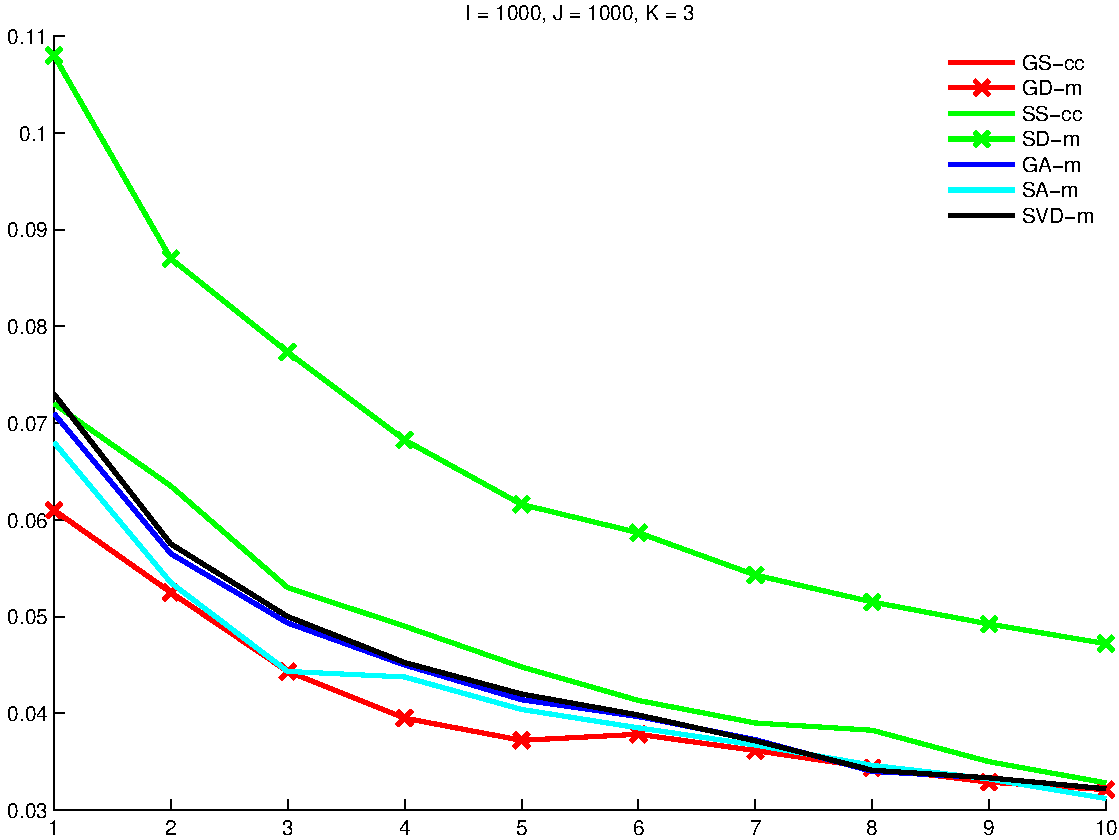
\includegraphics[scale=0.4]{figs/prec_DS1_I1000_J1000_1.pdf}&
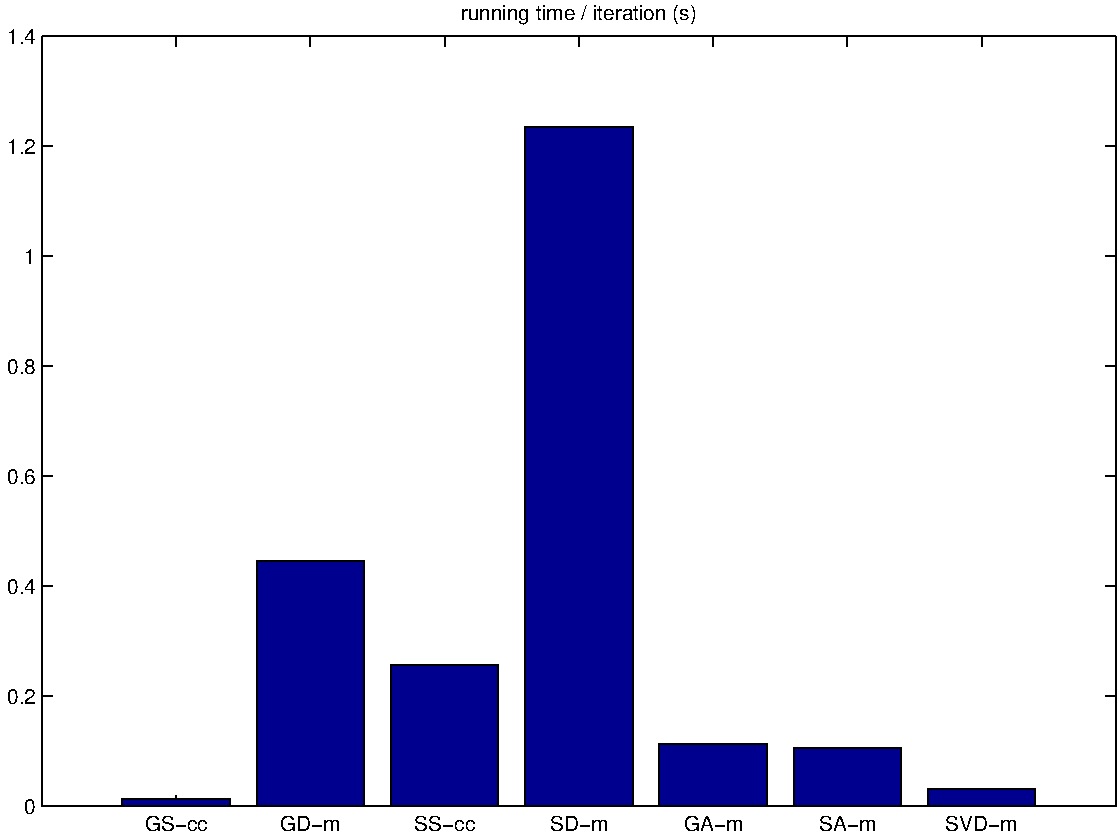
\includegraphics[scale=0.4]{figs/time_DS1_I1000_J1000_1.pdf}\\
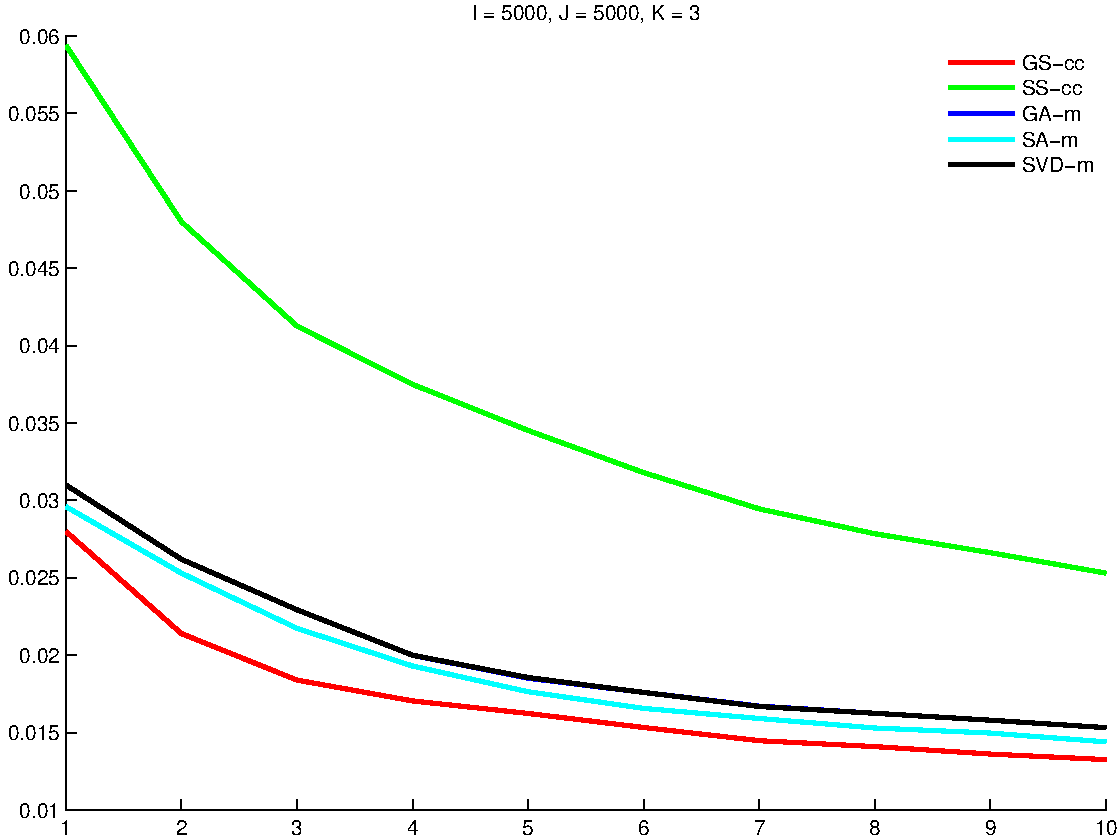
\includegraphics[scale=0.4]{figs/prec_DS1_I5000_J5000_1.pdf}&
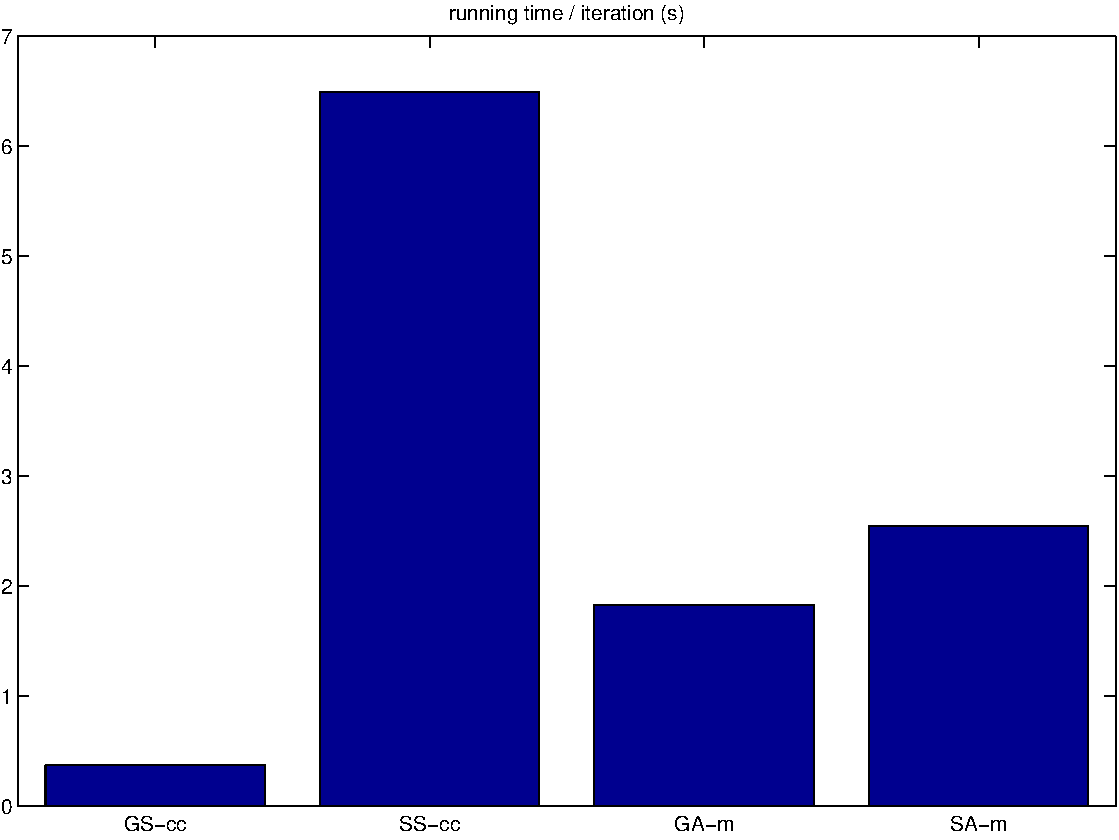
\includegraphics[scale=0.4]{figs/time_DS1_I5000_J5000_1.pdf}\\
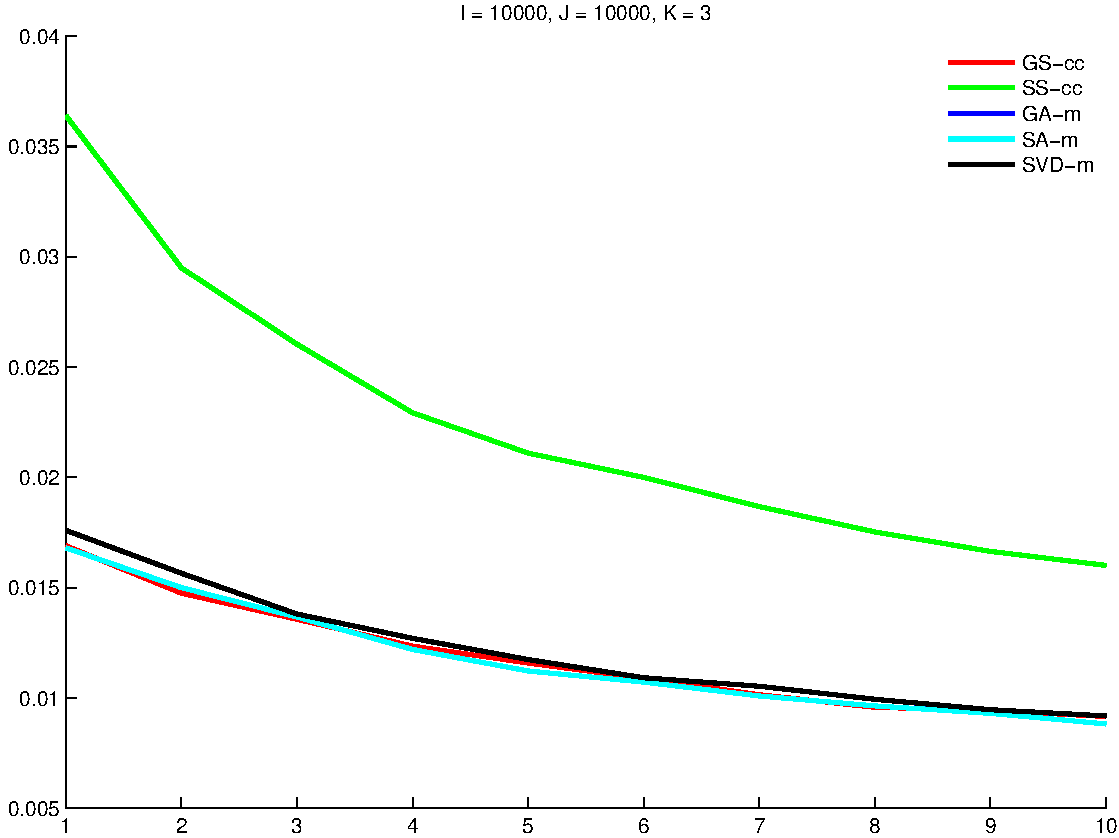
\includegraphics[scale=0.4]{figs/prec_DS1_I10000_J10000_1.pdf}&
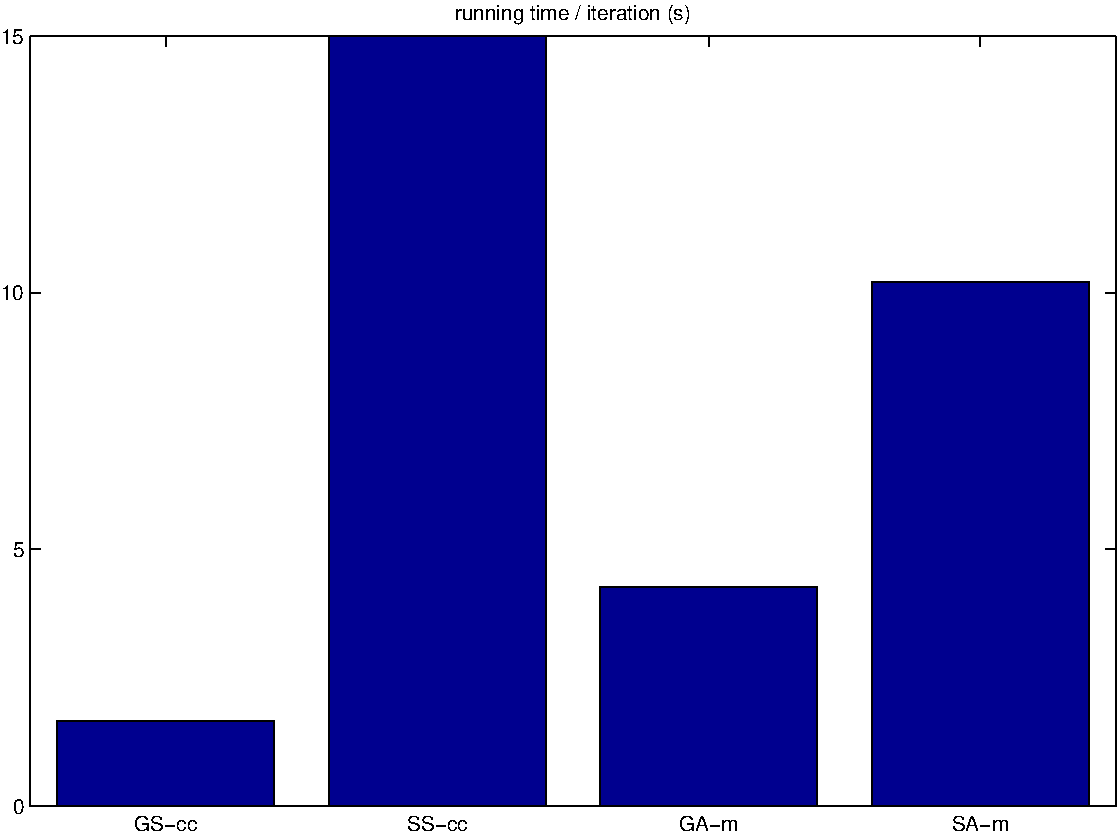
\includegraphics[scale=0.4]{figs/time_DS1_I10000_J10000_1.pdf}
\end{tabular}
\caption{Precisions and running times (per iteration) on artificial matrices.\label{fig:artificial_results}}
\end{figure}

Firstly, it can be observed that the Sigmoidal models with gradient descent significantly outperform the competitors. Secondly it can be seen that the sparse implementations are significantly faster than their dense counterparts. Finally, despite (on the small matrix), the sampling Sigmoid gradient descent algorithm 
being outperformed by the full counterpart on the small dataset, 
it still outperforms all the others on the larger datasets, with comparable running times.
A nice feature is that the number of samples can be tuned to trade of performance with computational time.

\subsection{Extensions and Real Datasets}

Before running experiments on real datasets, performance of the gradient descent algorithms can
be improved by adding a couple of `bells and whistles'.
Firstly every row and column can be given its own specific `offset' parameter, similar to $b$.
This can be added directly into the model by adding an additional column/row of parameters and
a column/row of ones to $\A$ and $\s$ respectively.

Secondly, the restriction of a zero-mean spherical prior needn't be maintained,
one can assign each parameter a prior of the form $p(a_{ik})=\N(a_{ik}|m_{a_{ik}},v_{a_{ik}})$.
The parameters of the prior can also be optimised to maximise the free energy also.

The analytic solution does not currently cater to either of these extensions.
We apply the first extension to the fast gradient descent algorithms

Results on a $2000\times 1000$ real dataset (Miguel, you sent me this dataset a while back, 
is it basket data?) are presented in Figure \eqref{fig:real_results}. 
Interestingly, on this dataset the additional row and column-wise offsets assist (SS), but not
(GS). Although the running times are a little slower (SS) and (SSe) 
yield by far the best performance.

\begin{figure}[h!]
\centering
\begin{tabular}{cc}
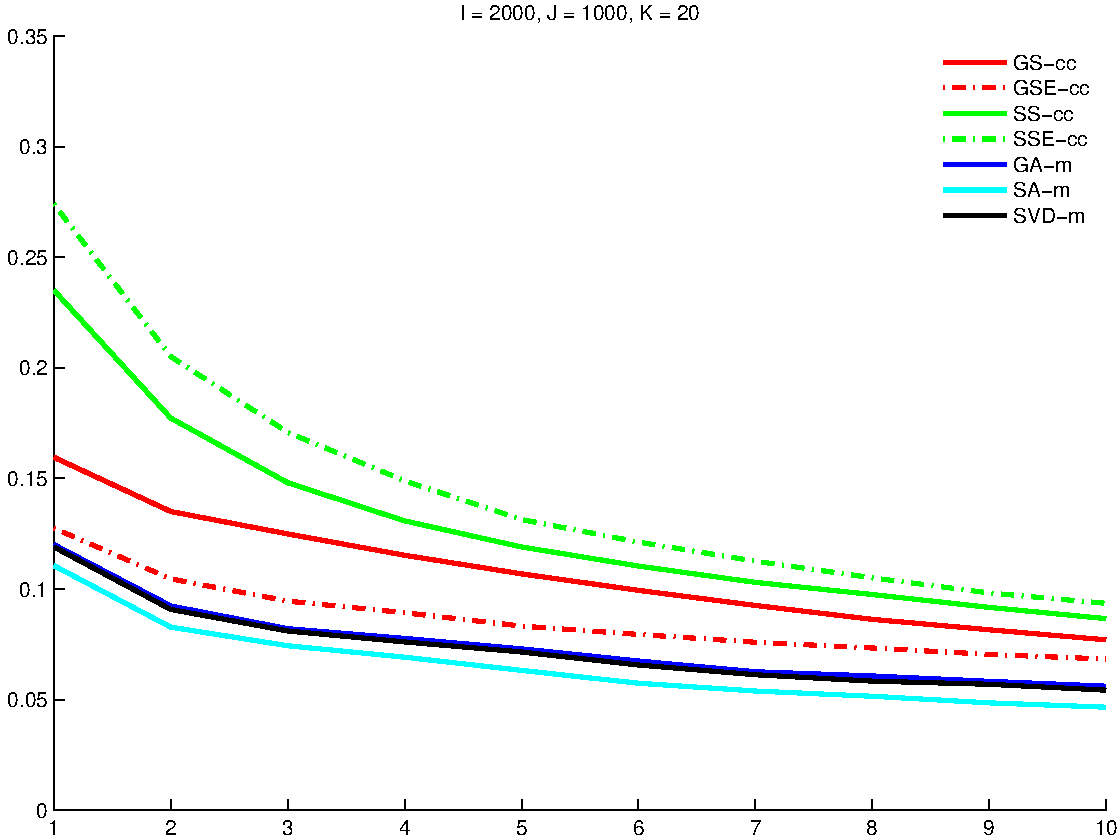
\includegraphics[scale=0.4]{figs/prec_DS2_I2000_J1000_1.pdf}&
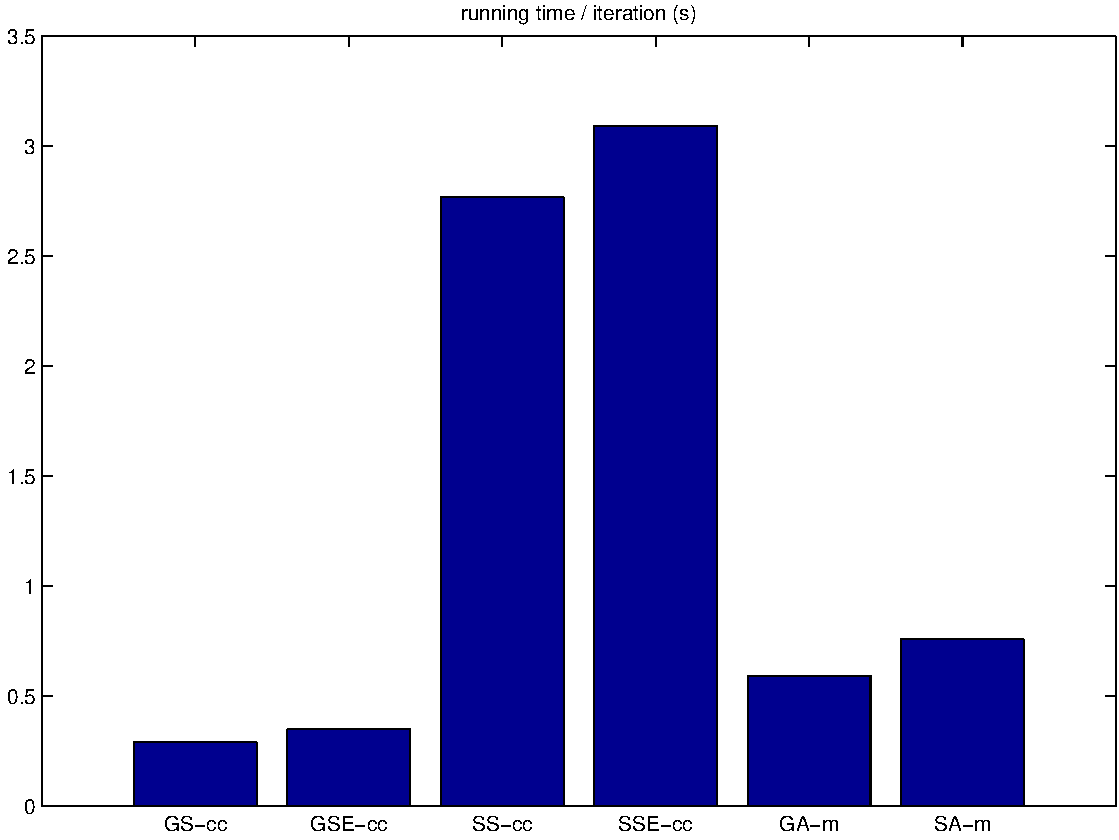
\includegraphics[scale=0.4]{figs/time_DS2_I2000_J1000_1.pdf}
\end{tabular}
\caption{Precisions and running times (per iteration) on real matrix.\label{fig:real_results}}
\end{figure}

NOTE: running time per iteration may be unfair, as typically most iterations are required for 
the Gaussian gradient descent based approaches, and least for (SA). (SA) requires only one iteration,
a single SVD, it is just included for the time being for comparison

\section{Future Work}\label{sec:future}

We can now factorise sparse binary matrices with up to $100M$ elements in just a few minutes.
However, one can add even more speed by changing the batch optimisation into a 
continuous, or batch approach \citep{hoffman2010}. TO IMPLEMENT.

Due to the fact that the priors can be inferred this algorithm could provide a core 
for a more sophisticated model. Suppose there are many matrices e.g. in a time series,
a GP prior could be places over the parameter matrices, and a alternating inference scheme 
could be employed.

\newpage
{
\bibliographystyle{apalike}
\bibliography{bibliog}
}

\end{document}
